\documentclass[a4paper]{article}

\usepackage[english]{babel}
\usepackage[utf8x]{inputenc}

\usepackage{amsmath}  % equations
\usepackage{cite}  % bibliograby
\usepackage{graphicx}  % images
\usepackage{pgfplots}  % plots
  \pgfplotsset{width=10cm,compat=1.9} % plots settings
  \usepgfplotslibrary{external}
  \tikzexternalize
\usepackage{todonotes}



\usepackage{hyperref}  % references
  \hypersetup{colorlinks=true,citecolor=black,filecolor=black,linkcolor=black,urlcolor=black} % references settings

\usepackage[automark]{scrpage2} % heading
  \pagestyle{scrheadings}
  \ihead[]{Handwritten character recognition in MPI} % left header
  \ohead[]{\today} % right header
  \cfoot[]{\pagemark} % footer
  \setheadsepline[122mm]{0.3mm}


% floor operator
\newcommand{\floor}[1]{\lfloor {#1} \rfloor}
\newcommand{\TODO}[1]{\noindent \textbf{\textcolor{red}{TODO: #1}}}


\begin{document}
	\title{
	\Huge Handwritten digit recognition
	}
	
	\vspace{2cm}
	
	\author{\Large \href{mailto:stefan.niculae@my.fmi.unibuc.ro}{Stefan Niculae} \and \Large \href{mailto:ionut.ciocoiu@my.fmi.unibuc.ro}{Ionut Ciocoiu}
	\vspace{3cm}}
	
	\date{
	\large Parallel \& Concurrent Programming Lab Report \\
    \vspace{0.2cm}
	\today
	}

	\maketitle
% 	\setlength{\parindent}{0pt}

\vspace{5cm}
\begin{abstract}
\TODO{rewrite when paper is done, talk about each section}

We implement a neural network to classify handwritten digits. The training is done in parallel, using MPI. We provide a comparison for model hyper-parameters and for training time vs number of processes. It achieves great accuracy and fast training time. An interactive demo is also presented
\end{abstract}



% \newpage
% \pagestyle{plain}
% \tableofcontents



\newpage
\section{Introduction}
\TODO{more here}


\section{Problem statement}
\label{sec:problem}
Pentru o retea neurala care foloseste un algoritm de antrenare bazat pe metoda gradientului descendent si dispune de o cantitate mare de date de antrenare timpul ca reteaua sa ajunga la rezultate satisfacatoare poate dura chiar si zile pe o implementare secventiala
Ne propunem sa elaboram o implementare paralela a metodei gradientului descendent. Vom folosi pentru validarea implementarii o problema celebra in computer vision, cea a detectarii cifrelor scrise de mana.

For a neural network witch use for training the gradient descendent algorithm and dispose a large amount of training data, the time to reach convergence it can take days in a sequentially implementation.
We purpose to elaborate a parallel implementation of gradient descendent, and for validate that we use a common problem in computer vision: given a picture of a handwritten digit, label it accordingly 0 - 9.

\section{Dataset}
\label{sec:dataset}
We demonstrate our model performance on the MNIST database, widely used dataset for training and testing in the field of machine learning. It contains 70 000 examples of labeled handwritten digits. The digits have been size-normalized and centered in a fixed-size image \cite{mnist}. 

\begin{figure}[htb]
\centering

\includegraphics[width=8cm]{images/mnist-images.png}
\caption{Sample MNIST images \cite{tf}}
\end{figure}


The images are black-and-white, with a resolution of $28 \times 28$ pixels, represented as an array of $784$ values. Each value ranges from $0$ to $1$ indicating the amount of blackness in the pixel.

\begin{figure}[htb]
\centering
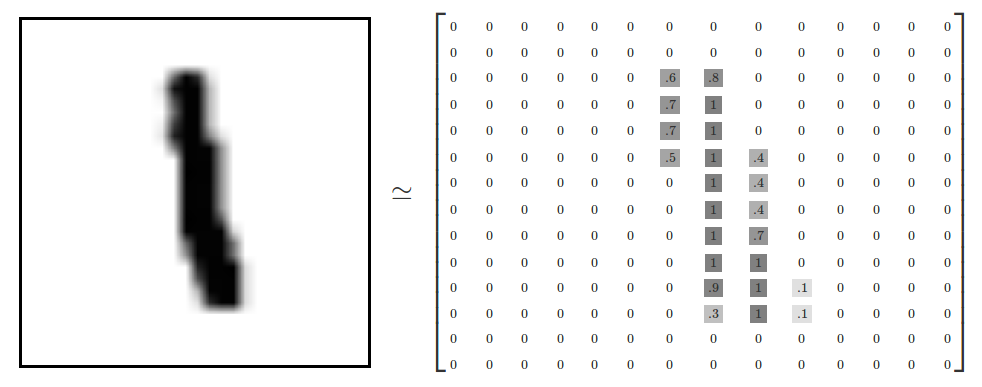
\includegraphics[width=8cm]{images/mnist-matrix.png}
\caption{Matrix representation of a digit \cite{tf}}
\end{figure}


\newpage
\section{Model}
\label{sec:model}
In order to recognize a given image, we need to model to understand the data. It needs to be able to be queried for a new instance in order to provide an interactive demo.
\\

We use a feed-forward neural network with an one fully connected layer, which predict the digit that has been in input image.
For an image $x$, initialy $28 \times 28$, we flatten this array into a vector of $784 = 28 \times 28$.


\begin{align}
y = softmax(Wx + b) \\
image\_label &= argmax(y)
\end{align}

In $(1)$, $W$ is the weights matrix, $10 \times 784$ -- the number of classes(one for each digit) and the dimension of an image ($784$). $b$ is the bias vector, $1 \times 10$, corresponding to the free element.
\\

The activation function output a vector of probabilities:
$$softmax(x_i)=\frac{exp(x_i)}{\sum_j exp(x_j)}$$
Where $exp(x)$ represents $e^x$, Euler's constant. It \textit{normalizes} the vector, causing the greatest elements to have logarithmic relative value.
\\

$(2)$ With $y$ vector of probabilities, $argmax$ take the index of the maximum value and results the prediction label.

\begin{figure}[htb]
\centering
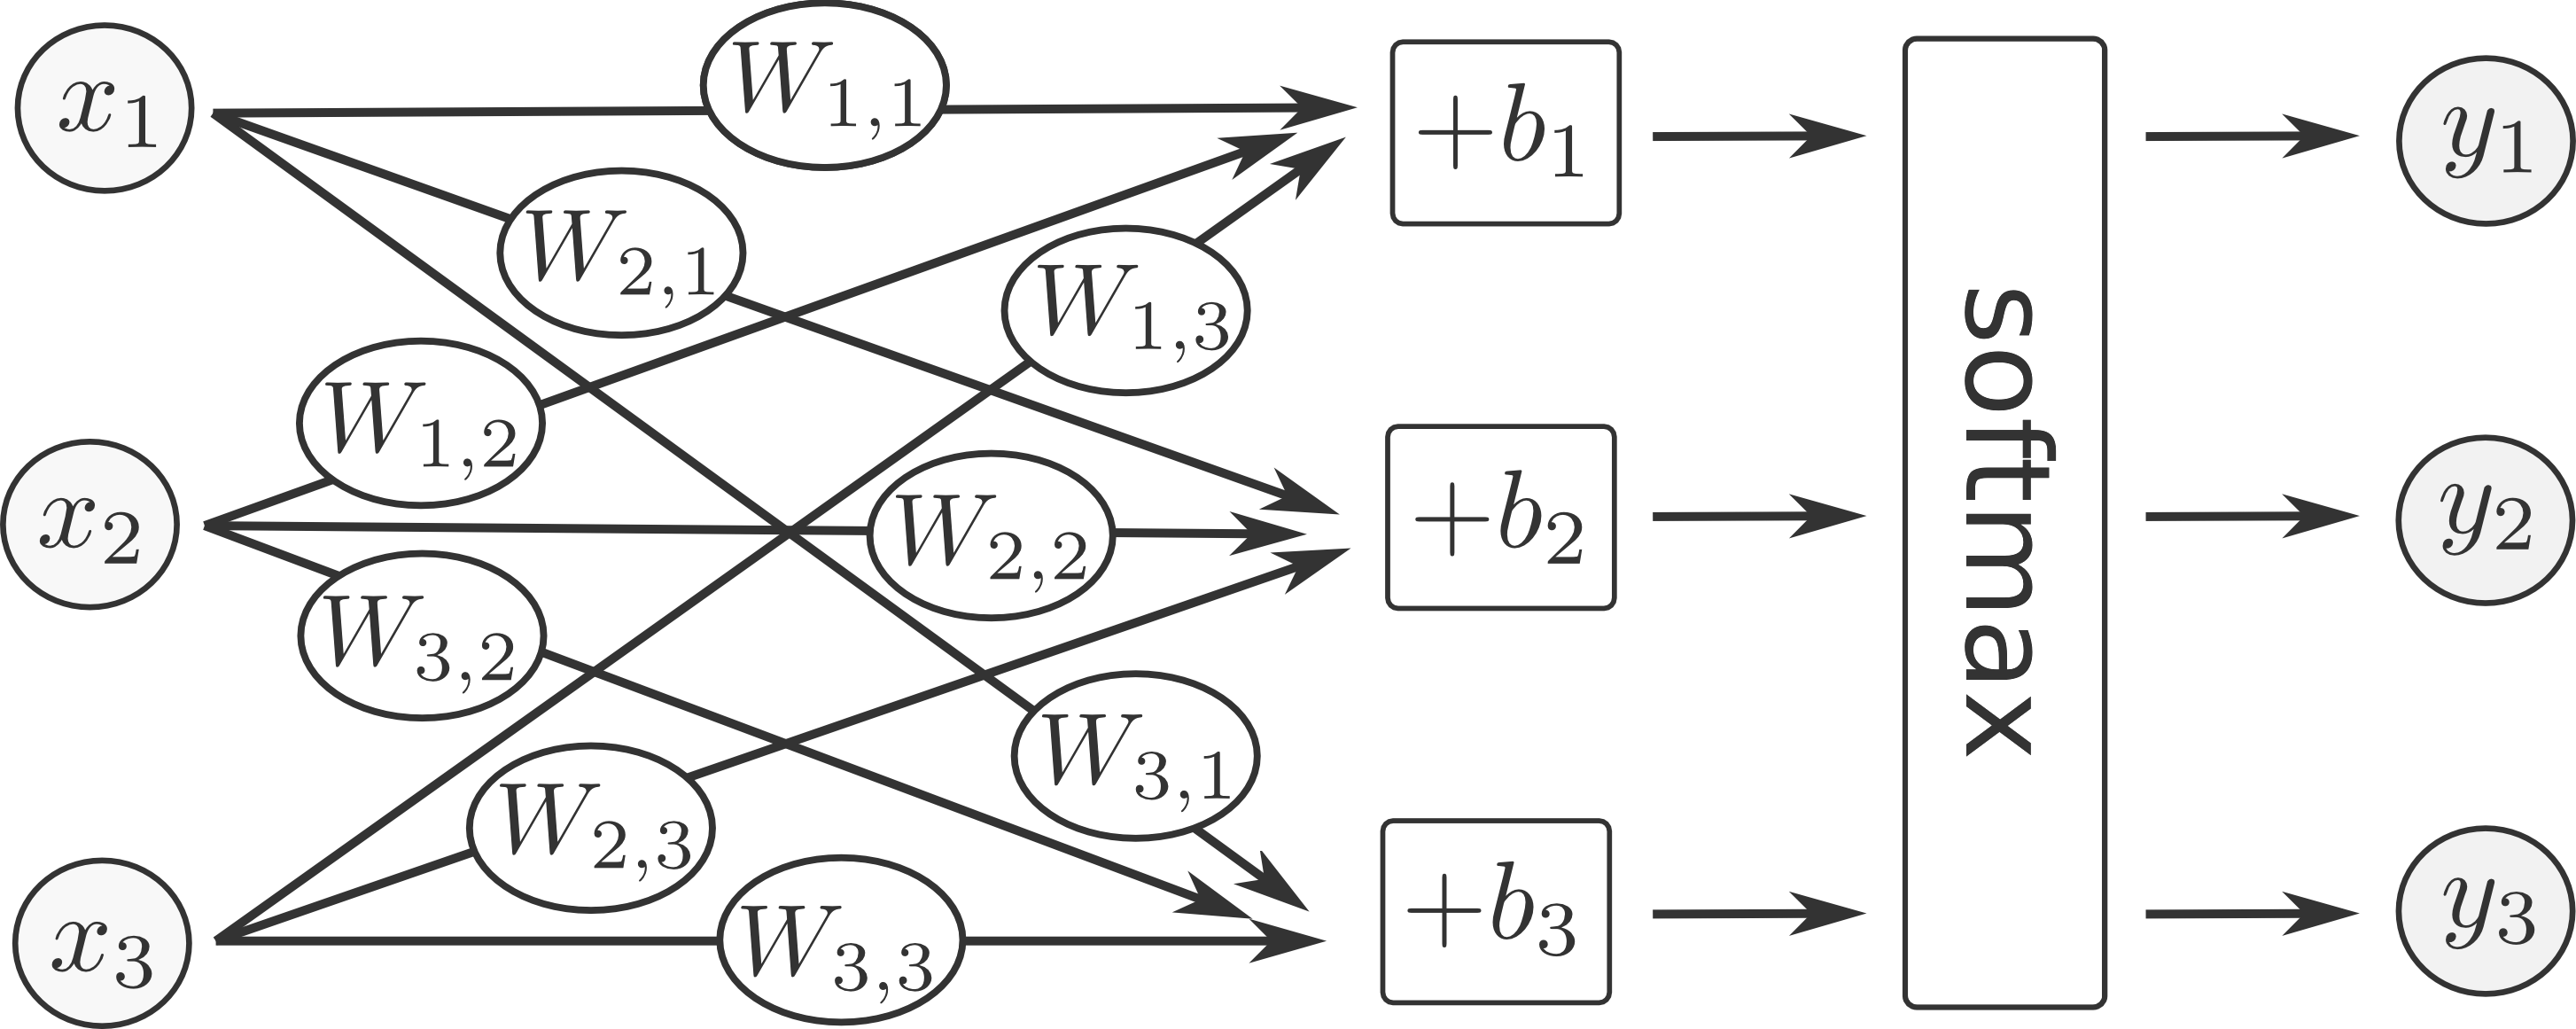
\includegraphics[width=8cm]{images/model-graph.png}
\caption{Simplified representation of model graph \cite{tf}}
\end{figure}

The cost function is cross-entropy:
$$H(y_t, y_p)=-\sum_x y_t log(y_p)$$
Where $y_t$ is the true, correct label of an image and $y_p$ is the label predicted by the model.
\\

$L_2$ regularization is used:
$$\frac{1}{\lambda} \sum_i \sum_j W_{i,j}^2$$
Where $\lambda$ is the regularization parameter. This limits overfitting by imposing a penalty on big weights.
\\

The model uses an adaptive learning rate:
$$\eta \frac{ W^{(k)} - W^{(k-1)} } { \nabla^{(k)} - \nabla^{(k-1)} }$$
Where $\eta$ is the momentum parameter. This helps with stability in late epochs.

\paragraph{Training} We employ gradient-descent on mini-batches. 
\begin{align*}
W^{(k)} &= W^{(k-1)} + \alpha \nabla_W^{(k-1)} \\ 
b^{(k)} &= b^{(k-1)} + \alpha \nabla_b^{(k-1)}
\end{align*}
Where $W$ is the weights matrix, $10 \times 784$ -- the number of classes( one for each digit) and the dimension of an image ($28 \times 28$). $b$ is the bias vector, $1 \times 10$, corresponding to the free element. $W^{(k)}$ denotes the weights at step $k$. $\nabla$ represents the update which must produce to improve prediction.
\\
Early-stopping prevents the model from further learning when performance on the validation split starts decreasing. Random sampling averts cycles when iterating through the dataset.

\paragraph{Evaluation}
Model performance is measured on a separate testing set using the accuracy metric -- ie: the percentage of images correctly classified.

\TODO{more about evaluation?}

\noindent The following chart illustrates model evolution, both on the test and on the training set, after each pass through the dataset.

\begin{center}
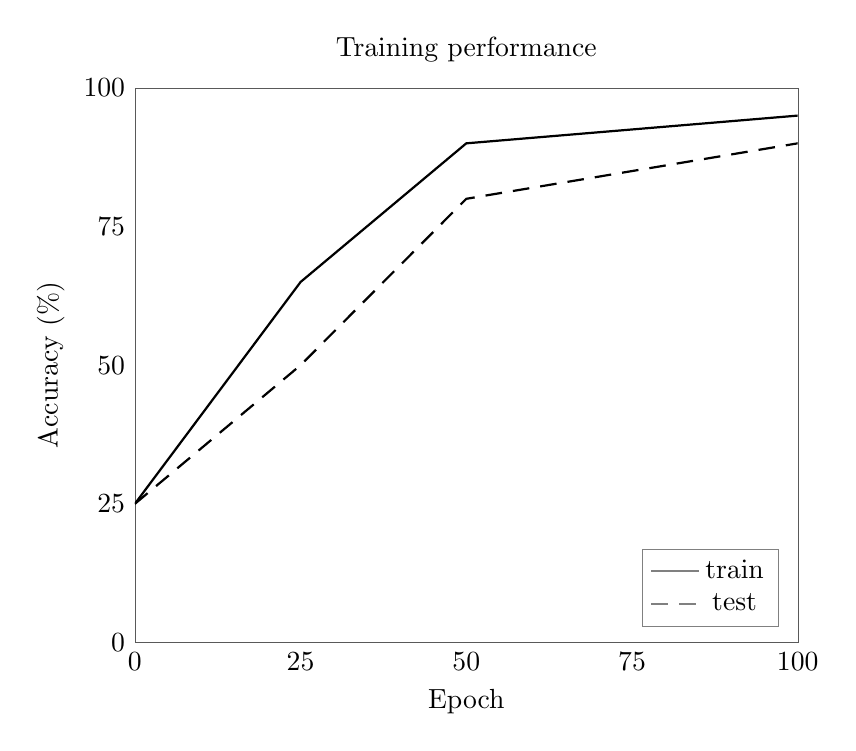
\begin{tikzpicture}
\begin{axis} [
  title={Training performance},
  xlabel={Epoch},
  ylabel={Accuracy (\%)},
  xmin=0, xmax=100,
  ymin=0, ymax=100,
  xtick={0,25,50,75,100},
  ytick={0,25,50,75,100},
  legend pos=south east,
  axis line style={black!65, line width=.1pt}, % thinner frame border
  legend style={draw=black!50, line width=.1pt}, % thinner frame border
  every x tick/.style={white}, % hide x ticks (make them white)
  every y tick/.style={white}, % hide y ticks (make them white)
  every axis plot/.append style={thick},
]

\addplot[]
  coordinates {
  (0,25)(25,65)(50,90)(100,95)
  };
\addplot[dash pattern=on 6pt off 4pt]
  coordinates {
  (0,25)(25,50)(50,80)(100,90)
  };
  
\legend{train, test}
\end{axis}
\end{tikzpicture}
\end{center}

\TODO{comment on chart}



\newpage
\section{Parallelization}
The phase that needs parallelization is the training of the model. Predicting is not computationally intensive. The bulk of the time is spent iterating over the entire training set multiple times. In one epoch, the network looks at every image, in batches and does the following:
\begin{itemize}
\item compute the change that must happen in order to better recognize -- called gradient,
\item updates its internal weights based on the gradient.
\end{itemize}
Computing the gradient takes the most time. The expensive operations are two dot-products on the weights matrices and the a matrix-wise softmax. This is the portion that we will parallelize.

When looking at a batch of images:
\begin{itemize}
\item the batch is assigned evenly among workers,
\item each worker computes the gradient on its chunk of the batch,
\item partial gradients are sent from each worker to the master,
\item the master process accumulates all the partial gradients and aggregates them,
\item the master updates the model weights based on the total gradient,
\item updated weights are sent back to every worker,
\item a new batch is ready to be processed: each worker now knows the effects of all the others.
\end{itemize}
In our case, aggregating the partial gradients requires nothing more then a summation.
\\

Naturally, there appears a running time -- model accuracy trade-off. Updating the weights after every image yields better accuracy than updating once every 1,000 samples. In the case of a greater batch size, the model has not evolved after looking at the first image, nor after the second or the third. It still analyzes them knowing just as much as it did when looking at the first sample.

In contrast, a greater batch size produces better parallelization performance. If each worker is assigned a single image, the communication cost of transferring gradient and weight matrices far outweighs the time taken to compute them. Efficiency improvement is present only when the time taken to transfer the results is lower than the time taken to compute them. Greater batch sizes incur more infrequent updates thus reducing the communication overhead.

The trade-off is now clear: a lower batch size leads to greater accuracy while a greater batch size causes faster training.
\\

Another approach would be to let the algorithm run sequentially and parallelize only the matrix multiplication operation. In light of the previously presented considerations, we can conclude that this would be grossly inefficient. The transfer overhead is much higher than the benefit gained by splitting the problem.

The following chart illustrates the improvement brought by parallelization on one pass through the data:

\begin{center}
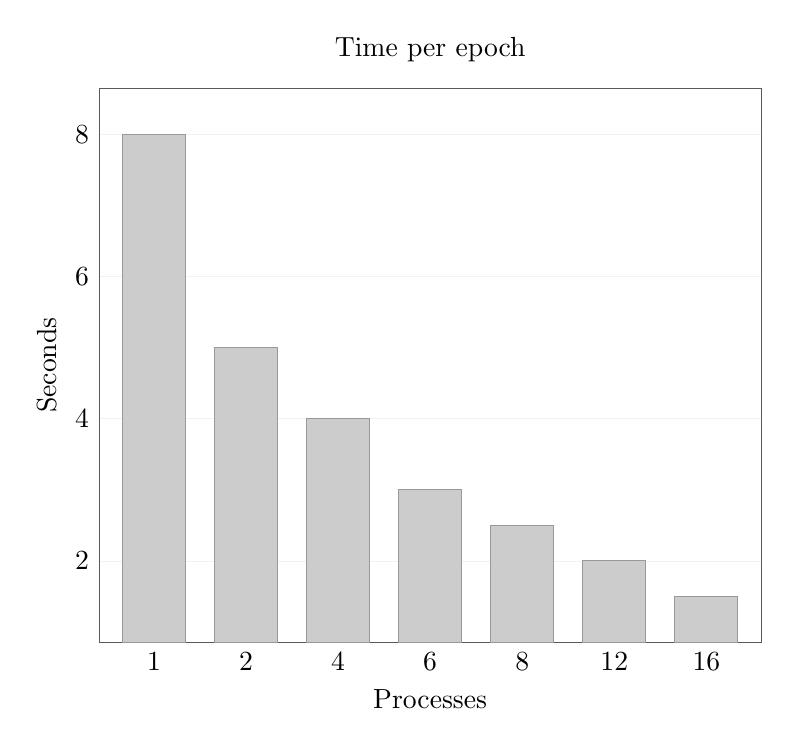
\begin{tikzpicture}
\begin{axis}[
  title={Time per epoch},
  xlabel=Processes,
  ylabel=Seconds,
  bar width=.8cm,
  axis line style={black!65, line width=.1pt}, % thinner border
  symbolic x coords={1,2,4,6,8,12,16}, % equidistant bars
  every x tick/.style={white}, % hide x ticks (make them white)
  every y tick/.style={line width=.1pt, draw=gray!10}, % y ticks same color as grid
  ymajorgrids=true, % show horizontal grid lines
  grid style={line width=.1pt, draw=gray!10}, % gray grid lines
  ]
  \addplot[ybar, black!40, fill=black!20] coordinates {
      (1,8) 
      (2,5)
      (4,4) 
      (6,3) 
      (8,2.5) 
      (12,2) 
      (16,1.5)    
      };
\end{axis}
\end{tikzpicture}
\end{center}

\TODO{comment on chart}

\newpage
\section{Graphical Interface}
The user is presented with a blank box in which to draw a digit to be recognized. Upon request, the prediction along with the model's confidence in it is displayed. 

\missingfigure[figcolor=white]{GUI}

\noindent Since the model was trained on $28 \times 28$ images, we need to pass the input in the same format. On today's screens, an input box of $28 \times 28$ pixels would look comically small. The raw input must be resized accordingly.

The simplest down-sizing method is taking each block of pixels in the original image and averaging it to form a single pixel in the resulting image. For simplicity, we assume square images and pixels with only one channel -- grayscale. Eg: an image with $n^2$ original pixels is condensed to $s^2$ pixels, meaning a factor of $f=\frac{n}{s}$. That means each of the $s^2$ pixels is a sum of a $f \times f$ block divided by $f^2$.

The trouble appears with encoding the image -- both the raw image and the model's inputs are in array form instead of a matrix. Ie: the pixels are all placed one after another starting from the top left corner.

\missingfigure[figcolor=white]{resizing example pdf}
The transformation can be computed by \textit{compacting} the columns:
$\sum_i Orig_i$ for column at index $\floor{\frac{i}{f}}$. Then for rows: $\sum_i Col_i$ for pixel at index $(i \bmod s) + \floor{\frac{i}{s \times f}}$. Where $Orig$ denotes the the original image $Col$ the column-wise averages. 







\newpage
\section{Implementation}
After going through the high-level overview of the project, we now delve into implementation details.

\paragraph{Predictive model} The core of the project is implemented in C++. This includes the neural network training and prediction. Model weights and image samples are kept in memory using 2D-arrays. 

Matrices build as vector of vectors (using the standard library implementation), while providing greater flexibility, cannot be sent efficiently using MPI. MPI deals with contiguous blocks of memory, while STL vectors are, by definition, dynamic. A work-around for this is to send a matrix row-by-row. Our initial implementation used this method but unfortunately it provides little to no increase in parallelization performance and caused a general-rewrite. 

The most expensive matrix operations are dot products and exponentiation. For matrix multiplication, we explored the Strassen algorithm, $O(n^{2.8})$, and the Coppersmith–Winograd algorithm, $O(n^{2.37})$. Although they achieve high asymptotic performance, hidden constants make them impractical in our case. We went with the Naive, $\Theta(n^3)$, algorithm with the $ikj$ optimization. For exponentiation, we rely on STL's implementation, although this can be further optimized.

\paragraph{Graphical Interface} The GUI is implemented as a web page in HTML, with a canvas for the input box.
The drawing is facilitated by the Sketch library \cite{sketch}. Interactivity and picture resizing is done through JavaScript.

\paragraph{Communication Server} The glue between the front-end and the model is a web-server done in Python, using the Flask library \cite{flask}. An array of $784$ pixels is received through from the GUI and is passed to the compiled executable. The output (predicted digit and prediction confidence) is then passed back through AJAX.
\\

\noindent The entire source code is available at \url{https://github.com/stefan1niculae/mnist-in-mpi}.

\vspace{\fill} % place references at the bottom
\bibliographystyle{ieeetr}
	\bibliography{references} % expects file "references.bib"
	\addcontentsline{toc}{section}{References}
    
    

\end{document}
